 \documentclass{beamer}
\usetheme{Madrid}

%==========Packages================
\usepackage[utf8]{inputenc}
    \usepackage[T1]{fontenc} 
    \usepackage[francais]{babel}
    \usepackage{amsmath}
    \usepackage{amssymb}
    \usepackage{graphicx}
    \usepackage{color}
    \usepackage{hyperref}
    \usepackage[left=2cm,right=2cm,top=2cm,bottom=2cm]{geometry}
    \usepackage{mathrsfs}
    \usepackage{verbatim}
   %========================================

\title{Application de chiffrement homomorphe à l'apprentissage automatique}

% A subtitle is optional and this may be deleted
    \subtitle{Optional Subtitle}
    \author{BENISSA Sami \\
      Université Paris 8\\
    Master Mathématiques fondamentales pour la protection de l'information}
\institute[Jolibrain, Toulouse, France] % (optional, but mostly needed)

\date{Jeudi 28 Septembre, 2017}

\AtBeginSection[]
{
  \begin{frame}<beamer>{Déroulement}
    \tableofcontents[currentsection]
  \end{frame}
}

\AtBeginSubsection[]
{
  \begin{frame}<beamer>{Déroulement}
    \tableofcontents[currentsection,currentsubsection]
  \end{frame}
}


\begin{document}

\begin{frame}
  \titlepage
\end{frame}

\begin{frame}{Déroulement}
  \tableofcontents
 
\end{frame}

\section{Présentation de l'entreprise}


%////////////SLIDE1\\\\\\\\\\\\\\\\\\
\begin{frame}{Présentation de l'entreprise}{Jolibrain, Toulouse}
\begin{itemize}
  \item {
    Vétérans de l'Intelligence artificielle et du Web\\
    +Expert
    \pause 
  }
  \item {   
    Open Source
    \pause
  }
    \item {   
      Machine Learning, Deep Learning, Reinforcement Learning, Stochastic Optimization, Search Enginesengin de recherche, system P2P \\
      etc...
    \pause
    }
\end{itemize}
\end{frame}
%\\\\\\\\\\\\\\\\\\\////////////////////

 %/////////////////NEW SLIDE\\\\\\\\\\\\\\\\\\
  

\section{Introduction}


%//////////////////////NEW SLIDE\\\\\\\\\\\\\\\\\
%\subsection{Contexte : Big data et Intelligence Artificielle}

\begin{frame}{Introduction}
\begin{block}{Contexte}
Big data et Intelligence Artificielle
\end{block}

%\subsection{Problématique : Ethique et confidentialité}

\begin{block}{Problématique}
Ethique et confidentialité.
\end{block}

%\subsection{Objectifs du stage}

\begin{block}{Objectif du stage}
Concevoir une application d'apprentissage automatique a partir des données chiffrées en utilisant un schéma de chiffrement homomorphe.
\end{block}
\end{frame}

%
%%%
\section{Etat de l'art}
  
%%%  

%////////////////////////NEW SLIDE\\\\\\\\\\\\\\\\\\\\

  \begin{frame}{Etat de l'art}

    \begin{itemize}
  \item {
    Cryptographie
  }
  \item {
    ML
  }
    \item {
    Cryptographie + ML
  }
  \end{itemize}
\end{frame}

  \subsection{Cryptographie}
  
  %////////////////////////NEW SLIDE\\\\\\\\\\\\\\\\\\\\
  %Chiffrement partiellement homomorphe définition
  \begin{frame}{Cryptographie}

    \begin{itemize}
    \item<1-> {
      Chiffrement partiellement homomorphe : Définition :\\
      \uncover<2->{Si on considère $C$ un cryptosystème,} \\

     \begin{itemize}[label={}]
           \item[]<3-> {
             $(x_1, x_2, ............, x_n)$ , l'ensemble de messages clairs, 
           }
           \item[]<4-> {  
             $(c_1, c_2, ..............., c_n)$ , l'ensemble des messages chiffrés
           }
           \item[]<5-> {
        et $ F$ une fonction de chiffrement telle que:\\
        $$F(x_n) = c_n$$
           }\\
     \end{itemize}

             \uncover<6-> {On dit que $C$ est homomorphique par rapport a l'addition si : \\
               $$F(x_1) + F(x_2) = F(x_1 + x_2).$$
                           }\\
      \uncover<7-> {On dit que $C$ est homomorphique par rapport a la multiplication si : \\
 $$F(x_1) * F(x_2) = F(x_1 * x_2).$$}
          }   
    
  \end{itemize}
\end{frame}

  %\\\\\\\\\\\\\\\\\\\\\\\\\\///////////////////////


   %////////////////////////NEW SLIDE\\\\\\\\\\\\\\\\\\\\
  %RSA, description
  \begin{frame}{Cryptographie}

    \begin{itemize}
    \item<1-> {
      RSA :\newline
      soient :\newline
      $pk = (n,e)$ :le clé publique.\newline 
      $sk = d$ : la clé secrète de cryptosystème.\newline
      $Enc$ : le fonction de chiffrement,\newline
      $Dec$ : la fonction de déchiffrement.\newline
      aon prend $c_1 = Enc(m_1) = m_1^e \;mod\;n$ et $c_2 = Enc(m_2) =m_2^e \;mod\;n$ 
              }
    \end{itemize}

  \end{frame}


  
 %\\\\\\\\\\\\\\\\\\\\\\\\\\///////////////////////


   %////////////////////////NEW SLIDE\\\\\\\\\\\\\\\\\\\\
  %Paillier, description
  \begin{frame}{Cryptographie}

    \begin{itemize}
    \item<1-> {
      Paillier :
              }
    \end{itemize}

  \end{frame}


  %//////////////NEW SLIDE\\\\\\\\\\\\\\\\\\\\\
  %Crypto completement homomorphe
  \begin{frame}{Cryptographie}

    \begin{itemize}
    \item<1-> {
      Chiffrement complètement homomorphe\\
      \uncover<2->{Un cryptosystème est dit homomorphe si une opération algébrique effectuée sur les chiffrés équivaut à une opération algébrique sur les clairs. En particulier, si le cryptosystème est stable pour un nombre arbitraire d'additions et de multiplications, il est dit complètement homomorphe.} \\
              }
    
  \end{itemize}
  \end{frame}
  %\\\\\\\\\\\\\\\\\\\·/////////////////////
  

  %//////////////NEW SLIDE\\\\\\\\\\\\\\\\\\\\\
  %Réseaux Euclidiens
  \begin{frame}{Cryptographie}

    \begin{itemize}
    \item<1-> {
      Réseaux Euclidiens : \\
      \uncover<2->{ Un réseau euclidien $L$ est un sous-groupe discret additif de $R^n$.\\
      }
      \uncover<3->{ une base $b= (b_1,b_2,...........,b_n)$ de $L$ dans $R^n$ est un ensemble de $n$ vecteurs linéairement indépendants.\\
        Les combinaisons linéaires entières des vecteurs de cette base forment $L$.
$$L = \{x\in R^n, tq\quad x = \sum_{i=1}^{n} x_ib_i,\quad x_i\in Z\}$$
      }
      \uncover<4->{\begin{figure}[h!]\begin{center}
                   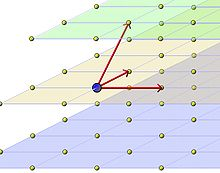
\includegraphics[width=3cm]{reseau.jpg}
                   \caption{Réseau euclidien de dimension 3 .}
                   \end{center}
                   \end{figure}
      }
      }
    
  \end{itemize}
  \end{frame}
  %\\\\\\\\\\\\\\\\\\\·/////////////////////

   %//////////////NEW SLIDE\\\\\\\\\\\\\\\\\\\\\
  %SVP et CVP
  \begin{frame}{Cryptographie}

    \begin{itemize}
    \item<1-> {
      \textbf{Shortest Vector Problem (SVP):}\\
      \uncover<2->{Etant donné une base $B$ d’un sous réseau $L$ de $Z^n$, trouver un vecteur non nul de $L$ le plus court possible pour la norme euclidienne.}\\
      \uncover<3->{
      \begin{figure}[h!]\begin{center}
          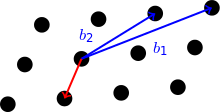
\includegraphics[width=3cm]{svp.png}
          \caption{En bleu la base donnée du réseau, en rouge le vecteur le plus court.}
    %\label{fig:svp}
        \end{center}
      \end{figure}
      }
    }
    \item<4->{
      \textbf{Closest Vector Problem (CVP):}\\
      \uncover<5->{Etant donné une base $B$ d’un réseau $L$ de $Z^n$ et un vecteur $v \in Q^n$ , trouver le vecteur de $L$ le plus proche de $v$ pour la norme euclidienne.}\\
      \uncover<6->{
        \begin{figure}[h!]\begin{center}
            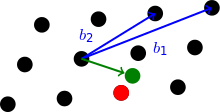
\includegraphics[width=3cm]{cvp.png}
            \caption{En bleu la base donnée du réseau, en vert le vecteur donné,en rouge le vecteur le plus proche du vecteur vert appartenant au réseau.}
            \label{fig:cvp}
          \end{center}
        \end{figure}
      }
    }
    \end{itemize}
  \end{frame}

  %//////////////NEW SLIDE\\\\\\\\\\\\\\\\\\\\\
  %Gentry
  \begin{frame}{Cryptographie}

    \begin{itemize}
    \item<1-> {
      \textbf{Cryptosystème de Gentry}\
      \uncover<2->{A toi de remplir} \\
              }
  \end{itemize}
  \end{frame}
  %\\\\\\\\\\\\\\\\\\\·/////////////////////
  
%//////////////NEW SLIDE\\\\\\\\\\\\\\\\\\\\\
  %BGV
  \begin{frame}{Cryptographie}

    \begin{itemize}
    \item<1-> {
      \textbf{Le cryptosystème Brakerski-Gentry-Vaikunthanathan (BGV)}\
      \uncover<2->{A toi de remplir} \\
              }
  \end{itemize}
  \end{frame}
  %\\\\\\\\\\\\\\\\\\\·/////////////////////


  \subsection{Apprentissage automatique}
 
%//////////////NEW SLIDE\\\\\\\\\\\\\\\\\\\\\
  %ML
  \begin{frame}{Apprentissage automatique}

    \begin{itemize}
    \item<1-> {
      \textbf{Apprentissage automatique \textit{Machine Learning - ML}}\\
      \uncover<2->{A toi de remplir} \\
              }
  \end{itemize}
  \end{frame}
  %\\\\\\\\\\\\\\\\\\\·/////////////////////

  \subsection{Cryptographie + ML}

  %//////////////NEW SLIDE\\\\\\\\\\\\\\\\\\\\\
  %BGV
  \begin{frame}{Apprentissage automatique}

    \begin{itemize}
    \item<1-> {
      \textbf{Crypto + ML}\\
      \uncover<2->{Pour certaines données sensibles, il n'est pas pensable d'effectuer des calculs sur le cloud. Pour pallier à ce problème de confidentialité et de sécurité, il est nécessaire de combiner ML et crypto} \\
      \uncover<3->{
        \begin{figure}[h!]\begin{center}
            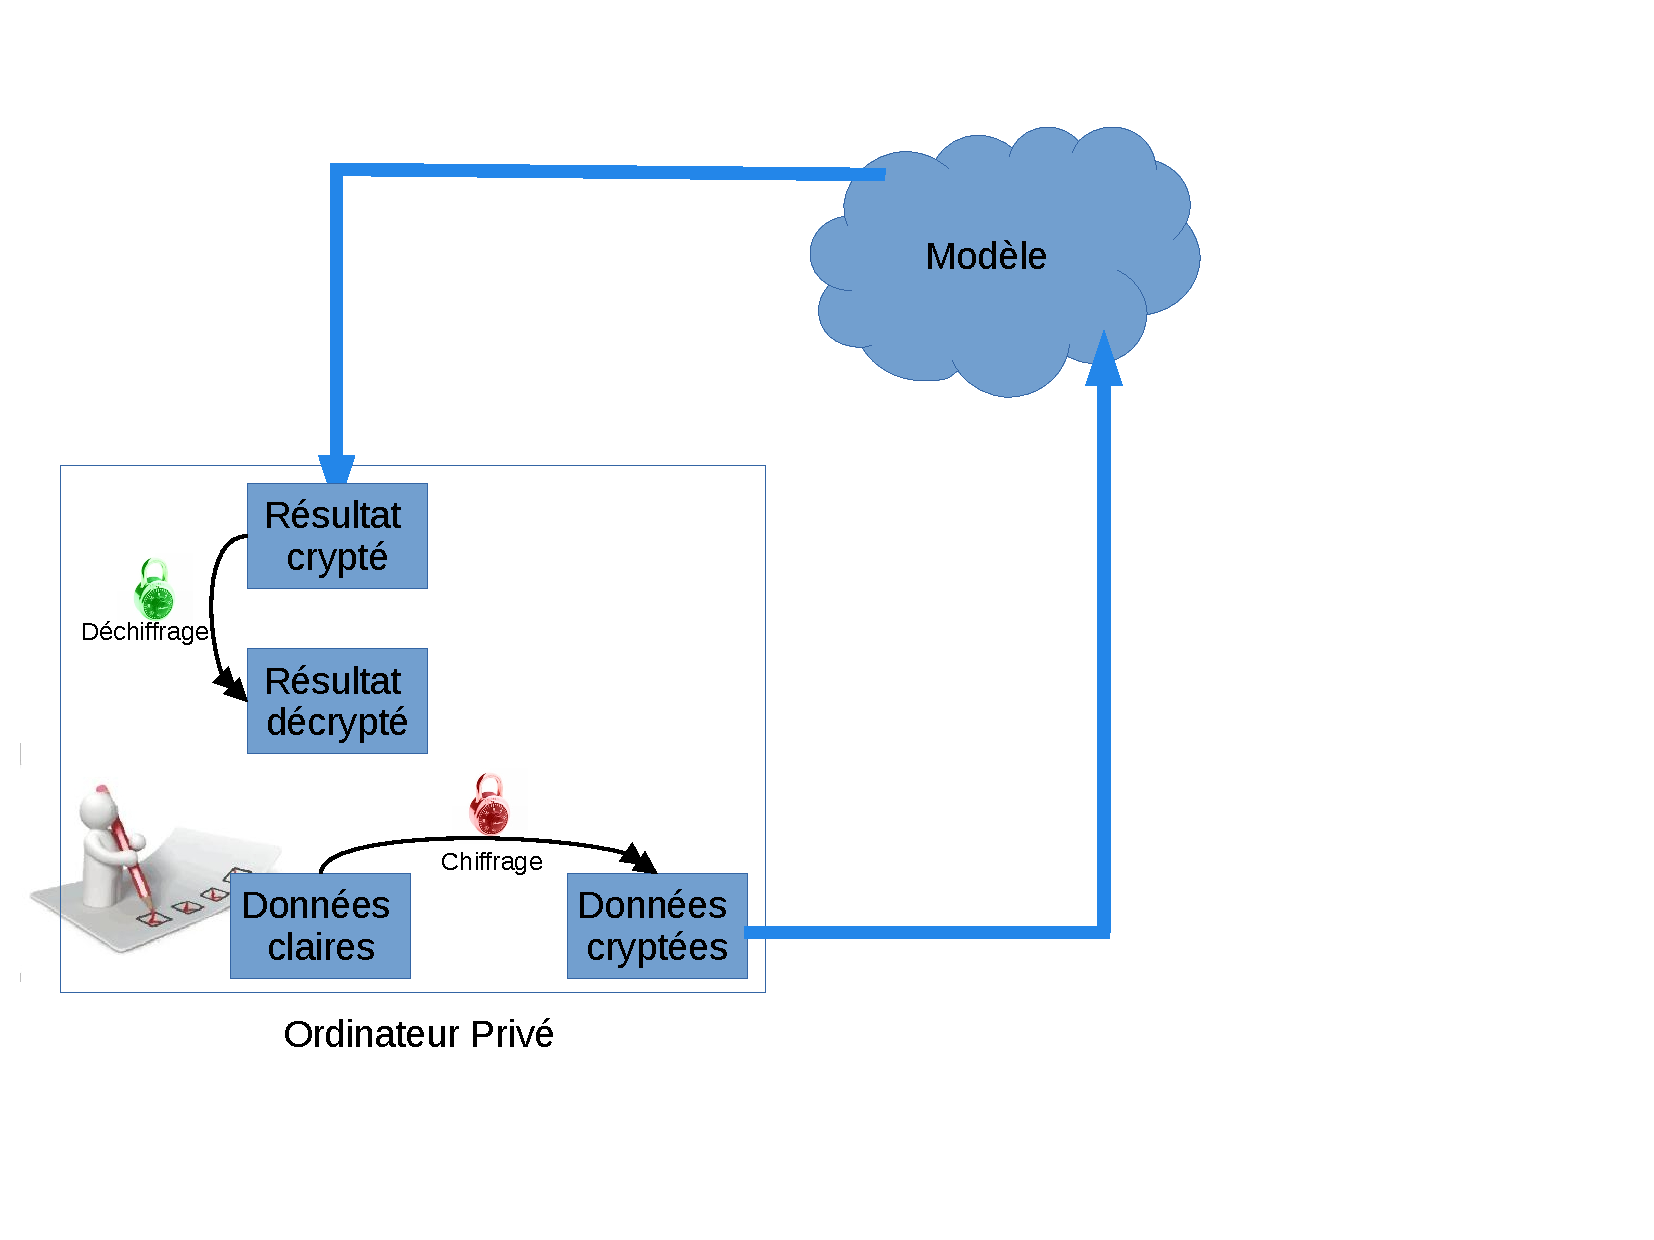
\includegraphics[width=5cm]{SchemaM1.pdf}
          \end{center}
        \end{figure}
      }
              }
  \end{itemize}
  \end{frame}
\section{Applications}
\subsection{Stochastic Gradient Descent(SGD)}
  \begin{frame}{Stochastic Gradient Descent(SGD)}
La descente de gradient stochastique, en machine learning elle premet de minimiser la fonction d'erreur, appliquable sur toutes fonction differentiables.\newline
\begin{block}{Algorithme}
\begin{enumerate}
	\item{choisir un point $x_0$.}
	\item{Itérer : 
\begin{itemize}
	\item{Calculer $\nabla f(x_t)$ }
	\item{Mettre à jour $x_{t+1}\leftarrow x_t - \alpha \nabla f(x_t)$}
\end{itemize}
	}
\end{enumerate}
\end{block}
\end{frame}
\subsection{Schéma explicative}
  \begin{frame}{Schéma explicative}
             \begin{figure}[h!]\begin{center}
             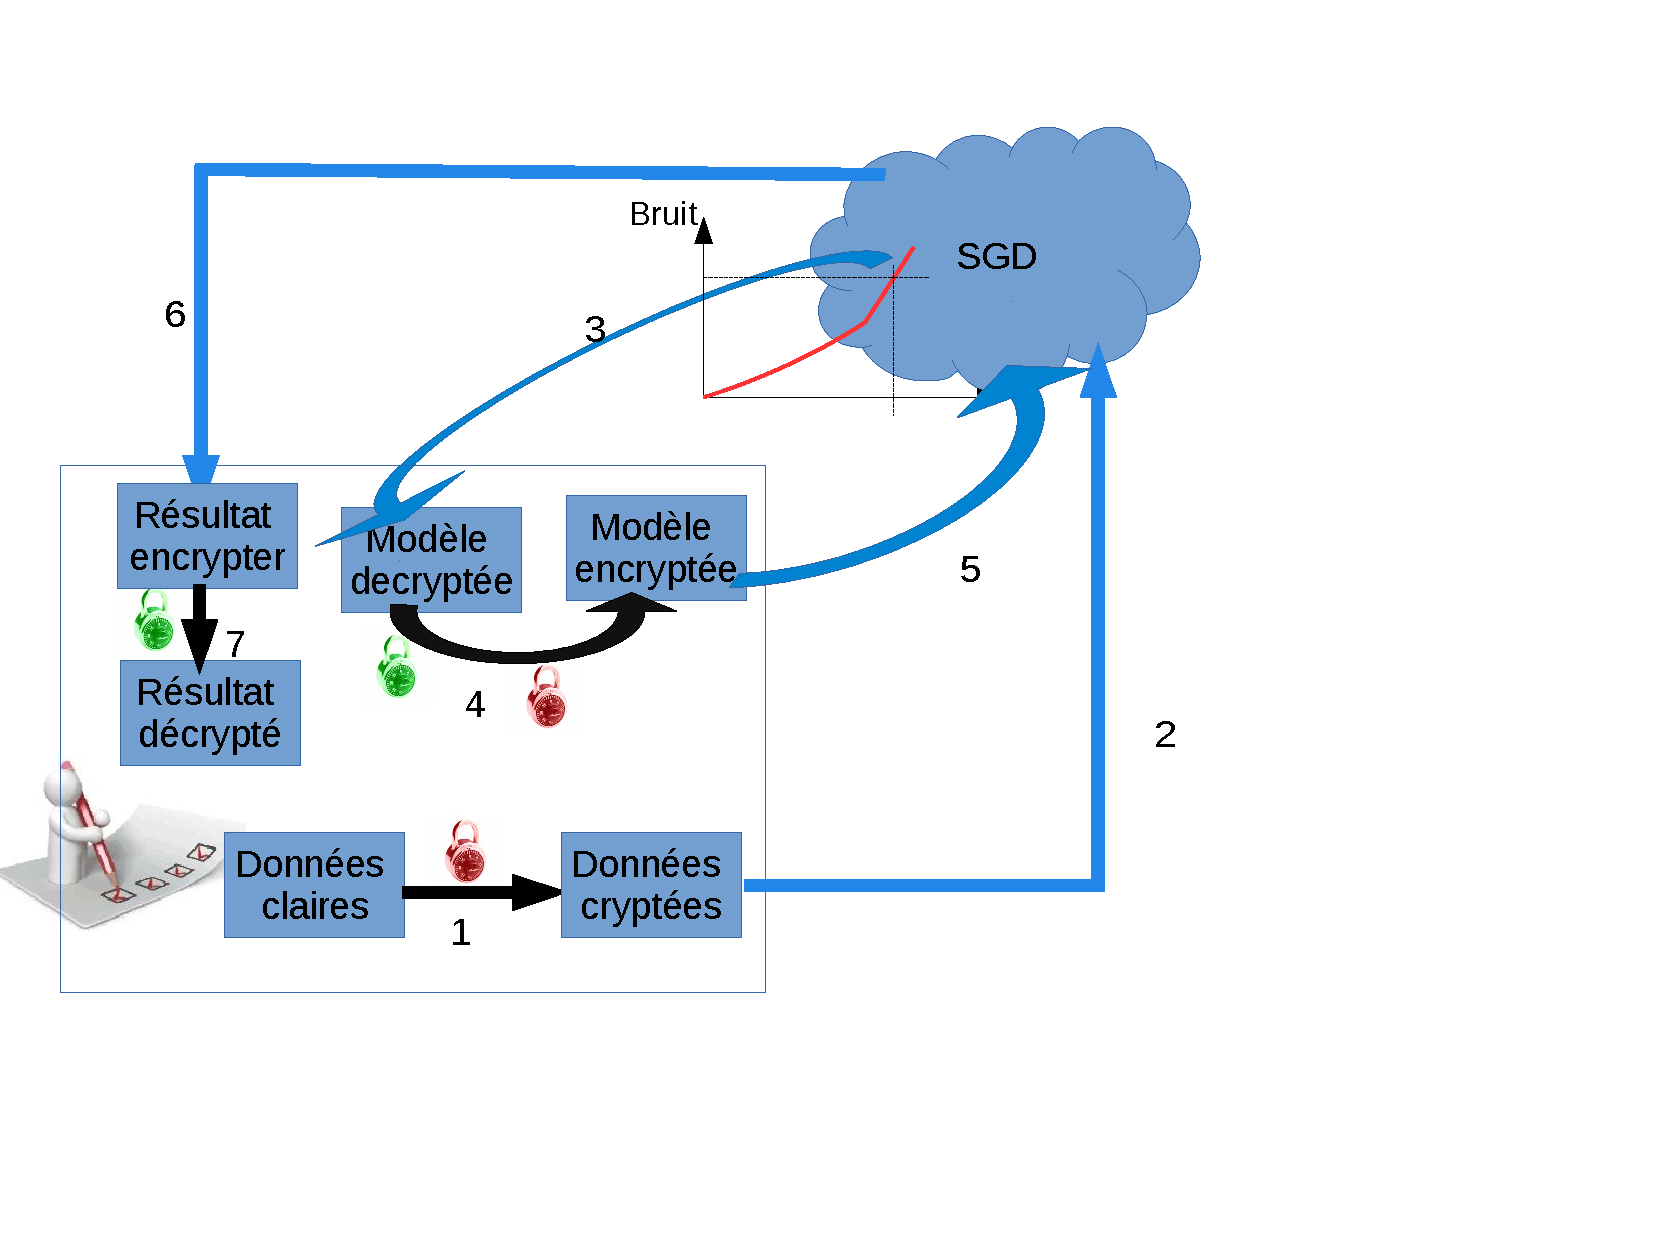
\includegraphics[width=10cm]{SGD.pdf}
             \end{center}
             \end{figure}
        \end{frame}
  \begin{frame}{Schéma explicative}
        \begin{enumerate}
    		\item {On chiffre les données sur lesquels on applique SGD (jeux de données, modèle) }
  			\item {On applique SGD sur les données, on met a jour le modèle, on calcul la fonction d'erreur après chaque itération. }
  			\item {Après un certain nombre d'itération on renvoit le modèle au déteneur de la clé secrète pour qu'il applique la fonction de 			       déchiffrement et la chiffrement pour repartir avec des données avec un bruit moins élevé. }
    		\item { A la fin on renvois le modèle chiffrés et on applique notre fonction de prédiction .}
		\end{enumerate}
  \end{frame}

\subsection{Approximation et résultats}
 \begin{frame}{Approximation et résultats}
 Dans la regression logistique on utilise la fonction sigmoid définie par :\newline
 $$f(x)=\dfrac{1}{1 + exp(-x)}$$
 Comme dans la bibliothèque SEAL la fonction exponentielle n'a pas été définie on a dû l'approximer avec :\newline
\begin{enumerate}
	\item{Developpement de Taylor}
	\item{Approximation avec piecewise function}
	\item{Fonction carré}
\end{enumerate}
\end{frame}
\subsubsection{Developpement de Taylor}
\begin{frame}{Developpement de Taylor}
On a :
\newcommand\omicron{o}
 $$\dfrac{1}{1+e^{-x}} = \dfrac{1}{2} + \dfrac{1}{4}x - \dfrac{1}{48}x^3 + \dfrac{1}{480}x^5 - \dfrac{1}{80640}x^7 + \omicron(x^9)$$
Dans un premier temps on a essayé de faire une approximation avec le developpement de Taylor, sauf qu'avec la fonction puissance (sous le nom exponentiate dans SEAL) on a un bruit qui s'accumule, et le texte chiffré devient vite indéchiffrable. 

\end{frame}
\subsubsection{Approximation avec piecewise function}
\begin{frame}{Approximation avec piecewise function}
Dans une deuxieme tentative on a approximé la fonction sigmoid avec la piecewise function qui est définie par :\newline
 \begin{equation}
f(x)=
\left\lbrace
\begin{array}{ccc}
0  & \mbox{si} & x<-2\\
1/2 + x/4 & \mbox{si} & -2<x<2\\
1 & \mbox{si} & x>2
\end{array}\right.
\end{equation}
Avec cette méthode on a réussi a avoir une fonction d'erreur (loss) qui converge de la même manière comme si on a travaillé avec des données non chiffrées comme il le montre la figure suivante :
\begin{figure}[h!]\begin{center}
             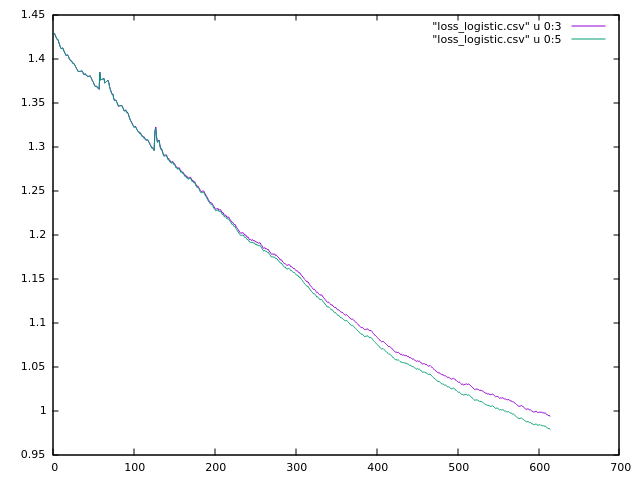
\includegraphics[width=4cm]{loss_logistic_regression.png}
             \end{center}
             \end{figure}

 \end{frame}
\subsubsection{Fonction carré}
\begin{frame}{Fonction carré}
\end{frame}
\begin{frame}
	\transdissolve<1>[duration=0.2]
	\begin{center}
	\textcolor{orange}{\textbf{\textit{Merci de votre attention.}}}
	\end{center}
\end{frame}


\end{document}


